\documentclass[10pt]{report}

\usepackage{graphicx}
\usepackage{caption}
\usepackage{subcaption}
\usepackage{listings}
\usepackage{float}
\usepackage{framed}
\usepackage{caption}

\begin{document}

\section{Capturing Data}
The image capture module is started by:
\begin{framed}
\begin{lstlisting}
$ roslaunch logitech_cam startup_camera2.launch
\end{lstlisting}
\end{framed}

Commands are generated and logged by:
\begin{framed}
\begin{lstlisting}
$ roslaunch logitech_cam logitech_cam_actuation.launch 
  command_generator_args:="-c [[50,0,0],[-50,0,0]] -t 
  600 -f 1" outfile:="~/captureddata/onlypan600.raw.ba
  g"
\end{lstlisting}
\end{framed}
This command will generate pan commands in each direction for 600 seconds and log the images and commands to the bag-file onlypan600.raw.bag


\section{Pre Processing}
The raw image stream is pre processed with pre\_processor.py. The following command gives an processed bag onlypan600.processed.bag with image size 160 time 120.
\begin{framed}
\begin{lstlisting}
$ rosrun logitech_cam pre_processor.py -i /home/adam/o
  nlypan600.raw.bag -o /home/adam/onlypan600.processed
  .bag -w 160 -h 120
\end{lstlisting}
\end{framed}


To validate that the processing worked as it should, one can view the processed image streams by:
\begin{framed}
\begin{lstlisting}
$ roslaunch logitech_cam show_processed.launch bagfile
  :="/home/adam/onlypan600.processed.bag"
\end{lstlisting}
\end{framed}

\section{Learning}
The learning is initialized by:
\begin{framed}
\begin{lstlisting}
$ rosrun logitech_cam learner.py -i /home/adam/onlypan
  600.processed.bag
\end{lstlisting}
\end{framed}

\section{Result}
\begin{figure}[H]
\centering
        \begin{subfigure}[b]{0.3\textwidth}
                \centering
                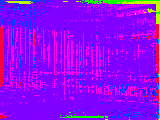
\includegraphics[width=\textwidth]{D0-angle.png}
                \caption{Phase Smooth}
                \label{fig:ps}
        \end{subfigure}
        \begin{subfigure}[b]{0.3\textwidth}
                \centering
                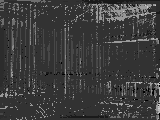
\includegraphics[width=\textwidth]{D0-norm.png}
                \caption{Modulus Smooth}
                \label{fig:tiger}
        \end{subfigure}
        \begin{subfigure}[b]{0.3\textwidth}
                \centering
                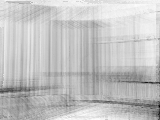
\includegraphics[width=\textwidth]{D0-variance.png}
                \caption{Variance Smooth}
                \label{fig:mouse}
        \end{subfigure}
        
        \begin{subfigure}[b]{0.3\textwidth}
                \centering
                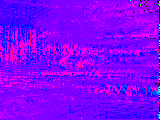
\includegraphics[width=\textwidth]{D0-angle-h.png}
                \caption{Phase}
                \label{fig:p}
        \end{subfigure}
        \begin{subfigure}[b]{0.3\textwidth}
                \centering
                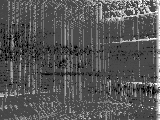
\includegraphics[width=\textwidth]{D0-norm-h.png}
                \caption{Modulus}
                \label{fig:m}
        \end{subfigure}
        \begin{subfigure}[b]{0.3\textwidth}
                \centering
                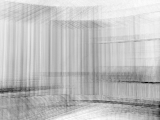
\includegraphics[width=\textwidth]{D0-variance-h.png}
                \caption{Variance}
                \label{fig:v}
        \end{subfigure}
        \caption{Diffeomorphism [500,0,0]}\label{fig:D0}
\end{figure}
\begin{figure}[H]
\centering
        \begin{subfigure}[b]{0.3\textwidth}
                \centering
                
\includegraphics[width=\textwidth]{D1-angle.png}
                \caption{Phase Smooth}
                \label{fig:ps}
        \end{subfigure}
        \begin{subfigure}[b]{0.3\textwidth}
                \centering
                
\includegraphics[width=\textwidth]{D1-norm.png}
                \caption{Modulus Smooth}
                \label{fig:tiger}
        \end{subfigure}
        \begin{subfigure}[b]{0.3\textwidth}
                \centering
                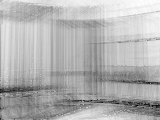
\includegraphics[width=\textwidth]{D1-variance.png}
                \caption{Variance Smooth}
                \label{fig:mouse}
        \end{subfigure}
        
        \begin{subfigure}[b]{0.3\textwidth}
                \centering
                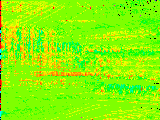
\includegraphics[width=\textwidth]{D1-angle-h.png}
                \caption{Phase}
                \label{fig:p}
        \end{subfigure}
        \begin{subfigure}[b]{0.3\textwidth}
                \centering
                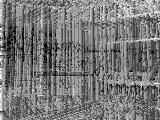
\includegraphics[width=\textwidth]{D1-norm-h.png}
                \caption{Modulus}
                \label{fig:m}
        \end{subfigure}
        \begin{subfigure}[b]{0.3\textwidth}
                \centering
                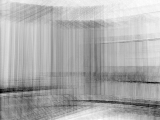
\includegraphics[width=\textwidth]{D1-variance-h.png}
                \caption{Variance}
                \label{fig:v}
        \end{subfigure}
        \caption{Diffeomorphism [-500,0,0]}\label{fig:D0}
\end{figure}




\end{document}
